\section{Radici di una funzione}

Data una funzione $f: [a,b] \subseteq \mathbb{R} \to \mathbb{R}$, vogliamo determinare un valore $x^* \in [a,b]$ tale che:
\[
f(x^*) = 0
\]
Diremo che $x^*$ è una \textbf{radice} (o uno \textbf{zero}) della funzione $f(x)$.

In generale, una radice $x^*$ può:
\begin{itemize}
    \item Esistere ed essere unica.
    \item Esistere ma non essere unica (es. $f(x) = \sin(x)$).
    \item Non esistere (es. $f(x) = e^x$).
\end{itemize}

I metodi che esamineremo, se la radice esiste, forniranno un'approssimazione di una di esse.  
Una caratteristica comune a tutti questi metodi è di essere di tipo \textbf{iterativo}:  
a partire da un'approssimazione iniziale $x_0$, viene prodotta una successione di approssimazioni $\{x_n\}_{n \ge 0}$ che, se il metodo è convergente, tende alla radice $x^*$:
\[
\lim_{n \to \infty} x_n = x^*
\]

\subsection{Il metodo di bisezione}
Il primo metodo che analizziamo è il metodo di bisezione.  
Si basa su due assunzioni fondamentali:
\begin{enumerate}
    \item La funzione $f(x)$ è \textbf{continua} in un intervallo chiuso e limitato $[a,b]$.
    \item Agli estremi dell'intervallo, la funzione assume valori di segno opposto, ovvero $f(a) \cdot f(b) < 0$.
\end{enumerate}

\begin{figure}[ht!]
    \centering
    \begin{tikzpicture}[scale=1.5]
        % Assi cartesiani
        \draw[->] (-0.5,0) -- (4,0) node[below] {$x$};
        \draw[->] (0,-1.5) -- (0,1.5) node[left] {$f(x)$};
        
        % Disegna la funzione
        \draw[thick, color=green!50!black] plot[smooth, domain=0.5:3.5] (\x, {cos(\x*60)+0.1*\x-0.5});
        
        % Punti e etichette
        \draw (1,0.05) -- (1,-0.05) node[below] {$a$};
        \draw (3,0.05) -- (3,-0.05) node[below] {$b$};
        \node[below, color=red] at (2.05, -0.05) {$x^*$};
        \fill[red] (2.05,0) circle (1.5pt);
        
        % Linee tratteggiate e valori
        \draw[dashed] (1,0) -- (1, {cos(60)+0.1*1-0.5});
        \draw[dashed] (0, {cos(60)+0.1*1-0.5}) -- (1, {cos(60)+0.1*1-0.5});
        \node[left] at (0, {cos(60)+0.1*1-0.5}) {$f(a) > 0$};
        
        \draw[dashed] (3,0) -- (3, {cos(180)+0.1*3-0.5});
        \draw[dashed] (0, {cos(180)+0.1*3-0.5}) -- (3, {cos(180)+0.1*3-0.5});
        \node[left] at (0, {cos(180)+0.1*3-0.5}) {$f(b) < 0$};
    \end{tikzpicture}
    \caption{Illustrazione del teorema degli zeri.}
    \label{fig:teorema_zeri}
\end{figure}

In base al \textbf{teorema degli zeri}, queste ipotesi garantiscono l'esistenza di almeno una radice $x^*$ nell'intervallo $(a,b)$.

Non sapendo dove si trovi $x^*$ all'interno di $[a,b]$, la migliore stima iniziale che possiamo fare è il punto medio dell'intervallo:
\[
x_1 = \frac{a+b}{2}
\]
A questo punto, si possono verificare tre casi:
\begin{enumerate}
    \item $f(x_1) = 0$: abbiamo trovato la radice.
    \item $f(a) \cdot f(x_1) < 0$: la radice si trova nell'intervallo $[a, x_1]$.
    \item $f(x_1) \cdot f(b) < 0$: la radice si trova nell'intervallo $[x_1, b]$.
\end{enumerate}
Ad ogni iterazione, l'ampiezza dell'intervallo di confidenza viene dimezzata.

\subsection{Implementazione e criteri di arresto}
Un'implementazione ``naive''\footnote{Per "implementazione naive" si intende una versione semplice e diretta dell'algoritmo che ignora problemi pratici di efficienza o stabilità numerica.} del metodo potrebbe essere:

\begin{lstlisting}
fa = f(a);
fb = f(b);
while true
    x1 = (a+b)/2;
    f1 = f(x1);
    if f1 == 0
        break;
    elseif fa*f1 < 0
        b = x1;
        fb = f1;
    else
        a = x1;
        fa = f1;
    end
end
\end{lstlisting}

Questo criterio di arresto non è robusto: a causa dell'aritmetica finita, la condizione `f1 == 0` potrebbe non verificarsi mai, anche se $x_1$ è molto vicino alla radice, portando a un ciclo infinito.

\paragraph{Esempio: Errore di valutazione}
Consideriamo il polinomio $p(x)=(x-1.1)^{20}(x-\pi)$, che ha una radice in $x=\pi$.  
Valutandolo in Matlab:
\begin{lstlisting}
p_coeffs = poly([1.1*ones(1,20), pi]);
polyval(p_coeffs, pi)
% ans = -5.5213e-05
\end{lstlisting}
Il risultato non è zero, e l'algoritmo naive andrebbe in loop.

\paragraph{Criterio basato sul numero di iterazioni}
Possiamo calcolare a priori il numero massimo di iterazioni necessarie per raggiungere una data tolleranza.  
Se $x_i$ è l'approssimazione al passo $i$, l'errore assoluto è maggiorato dalla semi-ampiezza dell'intervallo:
\[
|x^* - x_i| \le \frac{b_i - a_i}{2} = \frac{b-a}{2^i}
\]
Per garantire un'accuratezza `tol`, imponiamo:
\[
\frac{b-a}{2^i} \le \text{tol}
\quad \Rightarrow \quad
i \ge \log_2\!\left(\frac{b-a}{\text{tol}}\right)
\]
Il numero massimo di iterazioni sarà quindi:
\[
i_{\max} = \left\lceil \log_2\!\left(\frac{b-a}{\text{tol}}\right) \right\rceil
\]
\footnote{Questa formula calcola il numero massimo di iterazioni necessarie per garantire un errore inferiore a `tol`. L'operatore $\lceil \cdot \rceil$ (ceiling) arrotonda all'intero superiore.}

\begin{lstlisting}
fa = f(a);
fb = f(b);
imax = ceil(log2(b-a) - log2(tol));

for i = 1:imax
    x1 = (a+b)/2;
    f1 = f(x1);
    
    if f1 == 0
        break;
    elseif fa*f1 < 0
        b = x1;
        fb = f1;
    else
        a = x1;
        fa = f1;
    end
end
\end{lstlisting}

\paragraph{Criterio basato sul residuo (controllo efficace)}
Un criterio di arresto più efficiente si basa sulla "piccolezza" del valore della funzione, $|f(x)|$.  
Lo sviluppo di Taylor di $f(x)$ attorno alla radice $x^*$ è:
\[
f(x) = f(x^*) + f'(x^*)(x-x^*) + O(|x-x^*|^2)
\]
Dato che $f(x^*)=0$, otteniamo:
\[
|x-x^*| \approx \frac{|f(x)|}{|f'(x^*)|}
\]
e imponendo $|x-x^*| \le \text{tol}$, si ha:
\[
|f(x)| \le \text{tol} \cdot |f'(x^*)|
\]
Poiché $f'(x^*)$ non è noto, lo approssimiamo come:
\[
f'(x^*) \approx \frac{f(b_i)-f(a_i)}{b_i - a_i}
\]

\paragraph{Algoritmo di bisezione ottimizzato}
\begin{lstlisting}
% Versione ottimizzata del metodo di bisezione
fa = f(a);
fb = f(b);
imax = ceil(log2(b-a) - log2(tol));

for i = 1:imax
    x1 = (a+b)/2;
    f1 = f(x1);
    
    % Stima della derivata e criterio di arresto sul residuo
    df = abs(fb-fa)/(b-a);
    if abs(f1) <= tol*df
        break;
    end
    
    % Aggiornamento dell'intervallo
    if fa*f1 < 0
        b = x1; fb = f1;
    else
        a = x1; fa = f1;
    end
end
% x1 contiene la radice approssimata
\end{lstlisting}


\subsection{Ordine di Convergenza}
Abbiamo esaminato il metodo di bisezione, definito sotto le ipotesi $f \in C([a,b])$ e $f(a)f(b)<0$. L'errore $e_i = x^* - x_i$ al passo $i$ soddisfa:
$$ |e_i| \le \epsilon_i = \frac{b-a}{2^i} $$
con $\frac{\epsilon_{i+1}}{\epsilon_i} = \frac{1}{2}$, il che implica $\lim_{i \to \infty} \frac{\epsilon_{i+1}}{\epsilon_i} = \frac{1}{2}$.

\begin{definition}[Ordine di Convergenza]
Un generico metodo iterativo si dice \textbf{convergente} se $\lim_{i \to \infty} e_i = 0$.
Si dice che ha \textbf{ordine di convergenza $p$} se $p$ è il più grande numero reale positivo tale che esista una costante $C > 0$ (costante asintotica dell'errore) per cui:
$$ \lim_{i \to \infty} \frac{|e_{i+1}|}{|e_i|^p} = C < \infty $$
\end{definition}

Per $i$ sufficientemente grande, vale $|e_{i+1}| \approx C |e_i|^p$.
\begin{itemize}
    \item Affinché ci sia convergenza, deve aversi $p \ge 1$.
    \item Se $p=1$, la convergenza è \textbf{lineare}. In questo caso, per $i$ grande, abbiamo:
          \begin{align*}
              |e_{i+1}| &\approx C |e_i| \\
              |e_{i+2}| &\approx C |e_{i+1}| \approx C^2 |e_i| \\
              &\vdots \\
              |e_{i+k}| &\approx C^k |e_i| 
          \end{align*}
          Questa successione tende a zero per $k \to \infty$ se e solo se $C < 1$. Pertanto, un metodo di ordine 1 è convergente se e solo se la sua costante asintotica dell'errore è minore di 1.
    \item Se $p=2$, la convergenza è \textbf{quadratica}.
    
\end{itemize}

\begin{osservazione}
Il metodo di bisezione, se applicabile, è sempre convergente, ha ordine $p=1$ e costante asintotica $C=1/2$.
\end{osservazione}

Un ordine $p$ più elevato implica una convergenza più rapida. Confrontiamo due metodi con $C=0.1$ e $|e_0|=0.1$:

\begin{table}[ht!]
\centering
\caption{Confronto tra convergenza lineare e quadratica ($|e_{i+1}| \approx C|e_i|^p$)}
\begin{tabular}{ccc}
\toprule
$i$ & Errore ($p=1$) & Errore ($p=2$) \\
\midrule
0 & $10^{-1}$ & $10^{-1}$ \\
1 & $10^{-2}$ & $10^{-3}$ \\
2 & $10^{-3}$ & $10^{-7}$ \\
3 & $10^{-4}$ & $10^{-15}$ \\
\bottomrule
\end{tabular}
\end{table}
È evidente che è bene ricercare metodi di ordine più elevato.

\paragraph{Condizionamento del Problema}
Vogliamo determinare $x^*$ tale che $f(x^*) = 0$. Se invece abbiamo una soluzione perturbata $\tilde{x}$ tale che $f(\tilde{x}) \neq 0$, studiamo come la perturbazione sul valore $f(\tilde{x})$ influenza l'errore $|\tilde{x} - x^*|$.
Usando Taylor: $f(\tilde{x}) \approx f'(x^*)(\tilde{x} - x^*)$, da cui:
$$ |\tilde{x} - x^*| \approx \frac{|f(\tilde{x})|}{|f'(x^*)|} $$
Il fattore $K = \frac{1}{|f'(x^*)|}$ è il \textbf{numero di condizione} del problema.
\begin{itemize}
    \item Se $|f'(x^*)| \ >> 1$ (non vicino a zero), il problema è \textbf{ben condizionato}.
    \item Se $|f'(x^*)| \approx 0$, il problema è \textbf{mal condizionato}.
\end{itemize}

\begin{definition}[Molteplicità di una radice]
Una radice $x^*$ ha \textbf{molteplicità $m \ge 1$} se $f(x^*) = f'(x^*) = \dots = f^{(m-1)}(x^*) = 0$ e $f^{(m)}(x^*) \neq 0$.
Se $m=1$, la radice è \textbf{semplice}. Se $m>1$, la radice è \textbf{multipla}.
\end{definition}

\begin{osservazione}
L'approssimazione di una radice multipla dà origine ad un problema \textbf{sempre mal condizionato}.
\end{osservazione}

\subsection{Metodo di Newton}
Il metodo di Newton è un metodo iterativo che, a partire da un'approssimazione $x_0$, costruisce la successione $\{x_i\}$ utilizzando l'interpretazione geometrica della derivata.

L'equazione della retta tangente al grafico di $f(x)$ nel punto $(x_0, f(x_0))$ è data da $y - f(x_0) = f'(x_0)(x - x_0)$. La nuova approssimazione $x_1$ si trova intersecando questa retta con l'asse delle $x$ (retta di equazione $y=0$). Dobbiamo quindi risolvere il sistema:
\[
\begin{cases} 
y - f(x_0) = f'(x_0)(x - x_0) & \leftarrow \text{retta tangente} \\
y = 0 & \leftarrow \text{asse x}
\end{cases}
\]
Sostituendo $y=0$ nella prima equazione e chiamando la soluzione $x_1$, otteniamo:
$$ -f(x_0) = f'(x_0)(x_1 - x_0) $$
Da cui si ricava la nuova approssimazione:
$$ x_1 = x_0 - \frac{f(x_0)}{f'(x_0)} $$
In generale, iterando questo procedimento, si ottiene la formula del metodo di Newton:
$$ x_{i+1} = x_i - \frac{f(x_i)}{f'(x_i)}, \quad i=0, 1, \dots $$

% --- INSERISCI QUI IL GRAFICO ---
\begin{figure}[ht!] % Ho cambiato [h!] in [ht!] come suggerito dal warning
\centering
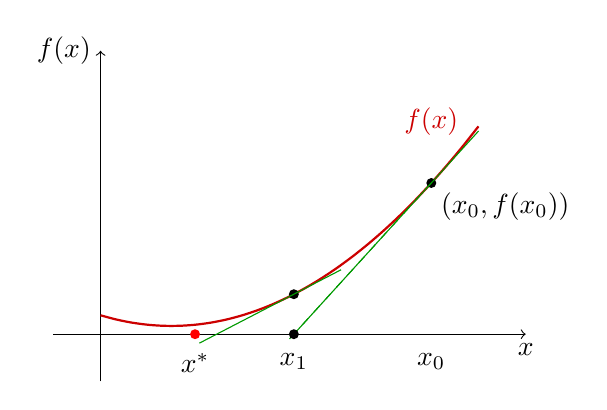
\begin{tikzpicture}[scale=1.2]
    % Assi
    \draw[->] (-0.5,0) -- (4.5,0) node[below] {$x$};
    \draw[->] (0,-0.5) -- (0,3) node[left] {$f(x)$};
    
    % Curva f(x)
    \draw[thick, color=red!80!black] plot[smooth, domain=0:4] (\x, {0.2*(\x-1)^2 + 0.1*\x});
    \node[above, color=red!80!black] at (3.5, 2) {$f(x)$};
    
    % Punto x0 e tangente
    \coordinate (x0) at (3.5, {0.2*(3.5-1)^2 + 0.1*3.5});
    \fill (x0) circle (1.5pt);
    \node[below right] at (x0) {$(x_0, f(x_0))$};
    \draw (3.5,-0.1) node[below] {$x_0$};
    
    % Calcolo della derivata in x0 (pendenza)
    % f'(x) = 0.4*(x-1) + 0.1 -> f'(3.5) = 0.4*2.5 + 0.1 = 1.1
    % Retta: y - f(x0) = 1.1 * (x - x0)
    \draw[color=green!60!black] (x0) -- +(-1.5, -1.5*1.1) coordinate (endtan0); % Disegna un pezzo della tangente
    \draw[color=green!60!black] (x0) -- +(0.5, 0.5*1.1); % Altro pezzo
    
    % Intersezione x1
    % y=0 => -f(x0) = 1.1 * (x1 - x0) => x1 = x0 - f(x0)/1.1
    % f(3.5) = 0.2*2.5^2 + 0.1*3.5 = 0.2*6.25 + 0.35 = 1.25 + 0.35 = 1.6
    % x1 = 3.5 - 1.6/1.1 = 3.5 - 1.4545... = 2.045...
    \coordinate (x1_inter) at (3.5 - 1.6/1.1, 0);
    \draw[dashed, color=green!60!black] (x0) -- (x1_inter);
    \draw (x1_inter)+(0,-0.1) node[below] {$x_1$};
    \fill (x1_inter) circle (1.5pt);

    % Punto x1 sulla curva e tangente
    \coordinate (x1) at (3.5 - 1.6/1.1, {0.2*((3.5 - 1.6/1.1)-1)^2 + 0.1*(3.5 - 1.6/1.1)});
    \fill (x1) circle (1.5pt);
    % f'(x1) = 0.4*(x1-1) + 0.1 = 0.4*(1.045...) + 0.1 = 0.418 + 0.1 = 0.518
    \draw[color=green!60!black] (x1) -- +(-1.0, -1.0*0.518);
    \draw[color=green!60!black] (x1) -- +(0.5, 0.5*0.518);
    
    % Intersezione x* (radice) - approssimata
    \coordinate (x_star) at (1,0); % f(1)=0.1, ma facciamo finta che sia la radice per semplicità
    \draw (x_star)+(0,-0.1) node[below] {$x^*$};
    \fill[red] (x_star) circle (1.5pt);

\end{tikzpicture}
\caption{Interpretazione geometrica del metodo di Newton.}
\label{fig:newton}
\end{figure}
% --- FINE GRAFICO ---

\paragraph{Considerazioni sul Metodo di Newton}
\begin{enumerate}
    \item È richiesta la derivabilità di $f(x)$ (almeno $f \in C^2$ in un intorno della radice per l'analisi).
    \item Il costo per iterazione è 1 valutazione di $f(x)$ e 1 valutazione di $f'(x)$.
\end{enumerate}

\begin{teorema}[Convergenza di Newton]
    Sia $f(x) \in C^{(2)}$ in un intorno della radice $x^*$. Supponiamo che il metodo di Newton converga a $x^*$, e che $x^*$ sia semplice. Allora l'ordine di convergenza è (almeno) 2.
\end{teorema}
\begin{proof}[Dimostrazione (schizzo)]
Sviluppando $f(x^*)$ in Taylor attorno a $x_i$:
$$ 0 = f(x^*) = f(x_i) + f'(x_i)(x^* - x_i) + \frac{1}{2} f''(\xi_i)(x^* - x_i)^2, \quad \xi_i \in (x_i, x^*) $$
Ponendo $e_i = x^* - x_i$ e $e_{i+1} = x^* - x_{i+1}$:
$$ 0 = f(x_i) + f'(x_i)e_i + \frac{1}{2} f''(\xi_i)e_i^2 $$
Dividendo per $f'(x_i)$ e usando $x_{i+1} = x_i - f(x_i)/f'(x_i)$:
$$ 0 = -(x_{i+1} - x_i) + e_i + \frac{1}{2} \frac{f''(\xi_i)}{f'(x_i)} e_i^2 $$
$$ 0 = -(x_{i+1} - x_i) + (x^* - x_i) + \frac{1}{2} \frac{f''(\xi_i)}{f'(x_i)} e_i^2 = (x^* - x_{i+1}) + \frac{1}{2} \frac{f''(\xi_i)}{f'(x_i)} e_i^2 $$
$$ e_{i+1} = - \frac{1}{2} \frac{f''(\xi_i)}{f'(x_i)} e_i^2 $$
Passando al limite per $i \to \infty$:
$$ \lim_{i \to \infty} \frac{|e_{i+1}|}{|e_i|^2} =  \frac{1}{2} \left|\frac{f''(x^*)}{f'(x^*)} \right| = C $$
Questo dimostra la convergenza quadratica ($p=2$).
\end{proof}

\begin{osservazione}[Radici multiple]
    Nel caso di una radice multipla, con molteplicità $m > 1$, si può dimostrare che:
    $$ \lim_{i \to \infty} \frac{|e_{i+1}|}{|e_i|} = \frac{m-1}{m} $$
    ovvero, l'ordine di convergenza del metodo di Newton diventa lineare ($p=1$), come conseguenza del mal condizionamento del problema.
\end{osservazione}

\subsection*{Riepilogo dei Metodi Visti}
\paragraph{Metodo di Bisezione}
\begin{itemize}
    \item Applicabile se $f \in C([a,b])$ e $f(a)f(b) < 0$.
    \item Ordine di convergenza lineare ($p=1$), con costante asintotica $C=1/2$.
    \item Il numero massimo di iterazioni per raggiungere una data accuratezza (\texttt{tol}) è noto a priori: $\text{imax} = \lceil \log_2(b-a) - \log_2(\text{tol}) \rceil$.
\end{itemize}

\paragraph{Metodo di Newton}
Formula iterativa: $x_{i+1} = x_i - \frac{f(x_i)}{f'(x_i)}$.
\begin{itemize}
    \item Richiede che $f(x)$ sia derivabile.
    \item Se $f \in C^2$ in un intorno di una radice semplice, allora si ha, se convergente alla radice, convergenza \textbf{quadratica} ($p=2$).
    \item Se converge a una radice \textbf{multipla} $x^*$ (molteplicità $m>1$), la convergenza è solo \textbf{lineare} ($p=1$) con $C = \frac{m-1}{m}$, riflettendo il mal condizionamento del problema.
\end{itemize}

\subsection{Convergenza Locale vs Globale}
A differenza del metodo di bisezione, per il metodo di Newton non è in generale possibile garantire la convergenza a partire da un punto iniziale $x_0$ qualsiasi.

\begin{esempio}[Non convergenza di Newton]
Consideriamo $f(x) = x^3 - 5x = x(x^2-5)$, che ha tre radici semplici: $0, \pm\sqrt{5}$. Applichiamo il metodo di Newton partendo da $x_0=1$.
$f'(x) = 3x^2 - 5$.
$$ x_1 = x_0 - \frac{f(x_0)}{f'(x_0)} = 1 - \frac{1^3 - 5(1)}{3(1)^2 - 5} = 1 - \frac{-4}{-2} = 1 - 2 = -1 $$
$$ x_2 = x_1 - \frac{f(x_1)}{f'(x_1)} = -1 - \frac{(-1)^3 - 5(-1)}{3(-1)^2 - 5} = -1 - \frac{-1 + 5}{3 - 5} = -1 - \frac{4}{-2} = -1 + 2 = 1 $$
La successione generata è $\{1, -1, 1, -1, \dots\}$, che evidentemente non converge.
\end{esempio}

% --- GRAFICO ESEMPIO NEWTON ---
\begin{figure}[H] % Usiamo [H] dal pacchetto float per forzare la posizione
\centering
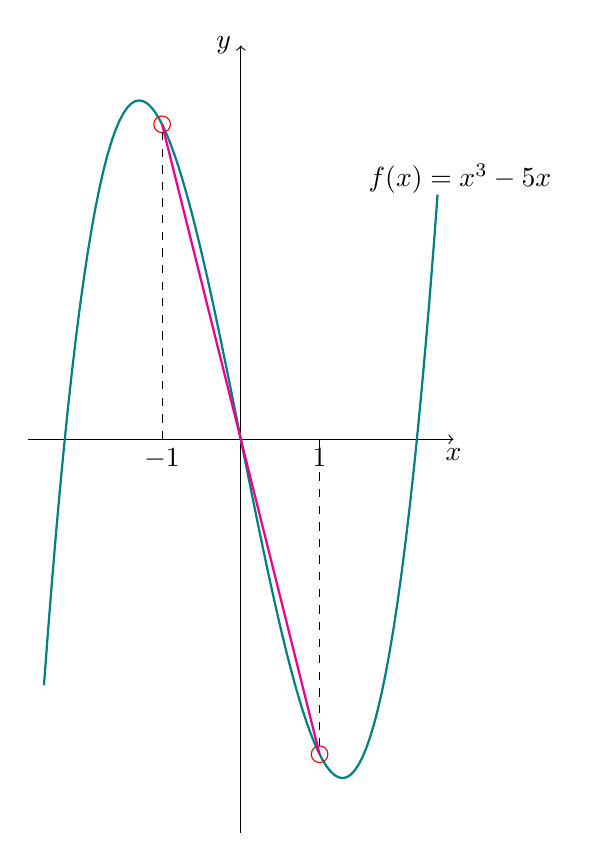
\begin{tikzpicture}[scale=1]
    % Assi
    \draw[->] (-2.7,0) -- (2.7,0) node[below] {$x$};
    \draw[->] (0,-5) -- (0,5) node[left] {$y$};
    \node[above right] at (1.5,3) {$f(x) = x^3 - 5x$};
    
    % Curva f(x)
    \draw[thick, color=teal, domain=-2.5:2.5, samples=100] plot (\x, {\x*\x*\x - 5*\x});
    
    % Punti x0=1 e x1=-1
    \coordinate (p1) at (1, -4);  % (1, f(1))
    \coordinate (m1) at (-1, 4);  % (-1, f(-1))
    
    % Cerchietti sui punti
    \draw[red] (p1) circle (3pt);
    \draw[red] (m1) circle (3pt);
    
    % Linee tratteggiate verticali
    \draw[dashed] (1,0) node[below] {$1$} -- (p1);
    \draw[dashed] (-1,0) node[below] {$-1$} -- (m1);
    
    % Tangenti (visualizzate come segmenti tra i punti)
    \draw[thick, color=magenta] (p1) -- (m1); 
    
\end{tikzpicture}
\caption{Metodo di Newton per $f(x)=x^3-5x$ partendo da $x_0=1$. Gli iterati oscillano tra 1 e -1.}
\label{fig:newton_oscillante}
\end{figure}
% --- FINE GRAFICO ---

La conclusione è che la convergenza del metodo di Newton è garantita solo in un opportuno \textbf{intorno} della radice. Si parla in questo caso di \textbf{convergenza locale}. Il metodo di bisezione, invece, ha \textbf{convergenza globale} (se applicabile, converge sempre).

\subsection{Teoria del Punto Fisso e Convergenza Locale}
Formalizziamo questo concetto per un generico metodo iterativo:
\begin{equation}
    x_{i+1} = \Phi(x_i), \quad i=0, 1, \dots
\end{equation}
dove $\Phi(x)$ è detta \textbf{funzione di iterazione}. Ad esempio, per Newton, $\Phi(x) = x - \frac{f(x)}{f'(x)}$.

Se il metodo serve a determinare la radice $x^*$ di $f(x)$, allora $x^*$ deve soddisfare la \textbf{proprietà di consistenza}:
\begin{equation}
    x^* = \Phi(x^*)
\end{equation}
ovvero, $x^*$ deve essere un \textbf{punto fisso} della funzione di iterazione $\Phi(x)$. Il problema di trovare uno zero di $f(x)$ è quindi equivalente a trovare un punto fisso di $\Phi(x)$.

Vogliamo capire sotto quali condizioni, partendo da un intorno del suo punto fisso, la successione (4) converge a $x^*$.

\begin{teorema}[del Punto Fisso / delle Contrazioni]
Sia $x^*$ un punto fisso di $\Phi(x)$. Se esiste $\delta > 0$ tale che per ogni $x, y \in I(x^*) = [x^*-\delta, x^*+\delta]$ la funzione $\Phi(x)$ è \textbf{Lipschitziana} con costante $L < 1$, cioè:
$$ |\Phi(x) - \Phi(y)| \le L |x - y| $$
allora:
\leavevmode % Aggiunto per risolvere potenziali conflitti
\begin{enumerate}
    \item Se $x_0 \in I(x^*)$, tutti i successivi iterati $x_i$ rimangono in $I(x^*)$ ($x_i \in I(x^*)$ per ogni $i \ge 0$).
    \item La successione $\{x_i\}$ converge a $x^*$.
\end{enumerate}
\end{teorema}
\begin{proof}
Dimostriamo per induzione che $x_i \in I(x^*)$. È vero per $i=0$. Supponiamo $x_i \in I(x^*)$. Allora:
$$ |x^* - x_{i+1}| = |\Phi(x^*) - \Phi(x_i)| \le L |x^* - x_i| $$
Poiché $L<1$ e $|x^* - x_i| \le \delta$, segue che $|x^* - x_{i+1}| < \delta$, quindi $x_{i+1} \in I(x^*)$.
Inoltre, applicando ricorsivamente la disuguaglianza:
$$ |x^* - x_i| \le L |x^* - x_{i-1}| \le L^2 |x^* - x_{i-2}| \le \dots \le L^i |x^* - x_0| $$
Dato che $L<1$, $L^i \to 0$ per $i \to \infty$, quindi $\lim_{i \to \infty} |x^* - x_i| = 0$.
\end{proof}

\begin{corollario}
    Se $\exists \delta > 0$ tale che $\forall x \in [x^*-\delta, x^*+\delta] = I(x^*)$ si ha $|\Phi'(x)| \le L < 1$, allora la successione $x_{i+1} = \Phi(x_i)$ converge a $x^*$ per $i \to \infty$.
\end{corollario}
\begin{proof}
Dal teorema del valor medio, per $x, y \in I(x^*)$, esiste $\xi$ tra $x$ e $y$ tale che:
$$ |\Phi(x) - \Phi(y)| = |\Phi'(\xi)(x-y)| = |\Phi'(\xi)| |x-y| \le L |x-y| $$
Quindi $\Phi(x)$ è Lipschitziana con costante $L<1$ e si applica il teorema precedente.
\end{proof}

\paragraph{Applicazione al Metodo di Newton}
Vediamo come si applica il risultato precedente al metodo di Newton. La funzione di iterazione è:
$$ \Phi(x) = x - \frac{f(x)}{f'(x)} $$
Verifichiamo la consistenza nel punto fisso $x^*$:
$$ \Phi(x^*) = x^* - \frac{f(x^*)}{f'(x^*)} = x^* - \frac{0}{f'(x^*)} = x^* $$
Calcoliamo ora la derivata prima di $\Phi(x)$:
$$ \Phi'(x) = \frac{d}{dx}\left(x - \frac{f(x)}{f'(x)}\right) = 1 - \frac{f'(x)f'(x) - f(x)f''(x)}{[f'(x)]^2} = \frac{[f'(x)]^2 - [f'(x)]^2 + f(x)f''(x)}{[f'(x)]^2} = \frac{f(x)f''(x)}{[f'(x)]^2} $$
Valutiamo la derivata nel punto fisso $x^*$:
\begin{itemize}
    \item \textbf{Se $x^*$ è una radice semplice}: In questo caso $f(x^*) = 0$ ma $f'(x^*) \neq 0$. Quindi:
    $$ \Phi'(x^*) = \frac{f(x^*)f''(x^*)}{[f'(x^*)]^2} = \frac{0 \cdot f''(x^*)}{[f'(x^*)]^2} = 0 $$
    Poiché $\Phi'(x^*) = 0 < 1$, per la continuità di $\Phi'(x)$, esisterà un intorno $I(x^*)$ tale che $|\Phi'(x)| \le L < 1$ per $x \in I(x^*)$. Di conseguenza, per il corollario precedente, il metodo di Newton converge localmente. Il fatto che $\Phi'(x^*) = 0$ è condizione sufficiente per la convergenza quadratica.
    
    % --- GRAFICO DERIVATA PHI ---
    \begin{figure}[H]
    \centering
    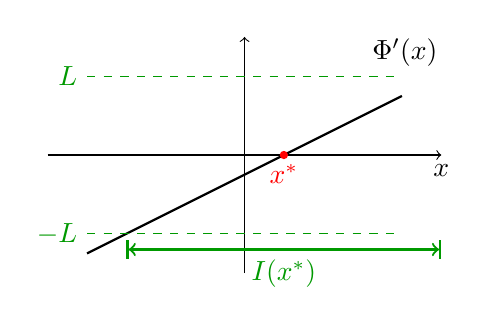
\begin{tikzpicture}[scale=1]
        % Assi
        \draw[->] (-2.5,0) -- (2.5,0) node[below] {$x$};
        \draw[->] (0,-1.5) -- (0,1.5) node[left] {}; % Asse y senza etichetta
        \node[above right] at (1.5,1) {$\Phi'(x)$};
        
        % Curva Phi'(x) passante per x* con derivata 0
        \draw[thick, domain=-2:2, samples=50] plot (\x, {0.5*(\x-0.5)}); % Curva generica con Phi'(x*)=0
        
        % Punto fisso x*
        \coordinate (xstar) at (0.5, 0);
        \fill[red] (xstar) circle (1.5pt);
        \node[below, red] at (xstar) {$x^*$};
        
        % Linee per L e -L (con L < 1)
        \draw[dashed, color=green!60!black] (-2,1) node[left] {$L$} -- (2,1);
        \draw[dashed, color=green!60!black] (-2,-1) node[left] {$-L$} -- (2,-1);
        
        % Intervallo I(x*) dove |Phi'(x)| < L
        % Trova i punti x tali che Phi'(x) = L e Phi'(x) = -L
        % 0.5*(x-0.5) = 1 => x-0.5=2 => x=2.5
        % 0.5*(x-0.5) = -1 => x-0.5=-2 => x=-1.5
        \draw[green!60!black] (-1.5, -1) -- (-1.5, {0.5*(-1.5-0.5)}); % Linea verticale sinistra
        \draw[green!60!black] (2.5, 1) -- (2.5, {0.5*(2.5-0.5)});    % Linea verticale destra (fuori asse)
                
        % Indicazione dell'intervallo sull'asse x
        \draw[|<->|,thick, green!60!black] (-1.5, -1.2) -- (2.5, -1.2) node[midway, below] {$I(x^*)$}; 
        
    \end{tikzpicture}
    \caption{Intorno $I(x^*)$ di una radice semplice dove $|\Phi'(x)| \le L < 1$, garantendo la convergenza locale.}
    \label{fig:phi_derivata_newton}
    \end{figure}
    % --- FINE GRAFICO ---

    \item \textbf{Se $x^*$ è una radice multipla} di molteplicità $m > 1$: Si può dimostrare che:
    $$ \Phi'(x^*) = \frac{m-1}{m} $$
    Anche in questo caso $|\Phi'(x^*)| < 1$, quindi il metodo converge ancora localmente (per il corollario). Tuttavia, poiché $\Phi'(x^*) \neq 0$, la convergenza diventa meno favorevole.
\end{itemize}
\subsection{Criteri di Arresto}
Per un metodo iterativo $x_{i+1} = \Phi(x_i)$, cerchiamo un criterio per fermare l'iterazione.

\paragraph{Criterio basato sul residuo}
Come visto per la bisezione, potremmo richiedere $|f(x_i)| \le \text{tol} \cdot |f'(x_i)|$ (approssimando $f'(x^*)$ con $f'(x_i)$). Dalla formula di Newton, questo è equivalente a:
$$ \left| \frac{f(x_i)}{f'(x_i)} \right| \le \text{tol} \implies |x_{i+1} - x_i| \le \text{tol} $$

\paragraph{Criterio basato sulla differenza tra iterati}
Il criterio $|x_{i+1} - x_i| \le \text{tol}$ controlla l'errore assoluto. Tuttavia, se $|x^*| \gg 1$, sarebbe più significativo controllare l'errore relativo:
$$ \frac{|x^* - x_i|}{|x^*|} \le \text{tol} $$
che può essere approssimato da:
$$ \frac{|x_{i+1} - x_i|}{|x_i|} \le \text{tol} \quad (\text{o } |x_{i+1}| \text{ al denominatore}) $$

\paragraph{Criterio combinato (auto-scalante)}
Un criterio pratico che combina i due è:
$$ |x_{i+1} - x_i| \le (1 + |x_i|) \cdot \text{tol} \quad \text{o equivalentemente} \quad \frac{|x_{i+1} - x_i|}{1 + |x_i|} \le \text{tol} $$
Questo criterio "auto-scalante" si comporta come un controllo sull'errore assoluto quando $|x_i| \approx 0$ e come un controllo sull'errore relativo quando $|x_i| \gg 1$, adattandosi alla grandezza della radice a cui si sta convergendo. \textbf{N.B.}: Da usare nei nostri elaborati.

\subsection{Metodi Quasi-Newton}
Ricordiamo che la derivata prima $f'(x_i)$ può essere approssimata dal rapporto incrementale:
$$ f'(x_i) \approx \frac{f(x_i+h) - f(x_i)}{h} $$
Se usassimo questa approssimazione con un $h$ fisso all'interno della formula di Newton, otterremmo una variante chiamata metodo \textbf{quasi-Newton}. Questo specifico approccio richiederebbe 2 valutazioni di funzione per iterazione ($f(x_i)$ e $f(x_i+h)$).

Per migliorare l'efficienza, possiamo usare le informazioni già calcolate nelle iterazioni precedenti.

\paragraph{Metodo delle Secanti}
Consideriamo la retta \emph{secante} passante per i punti $(x_{i-1}, f(x_{i-1}))$ e $(x_i, f(x_i))$. Il suo coefficiente angolare è:
$$ \frac{f(x_i) - f(x_{i-1})}{x_i - x_{i-1}} $$
Usiamo questo valore come approssimazione di $f'(x_i)$ nella formula di Newton. L'iterazione del \textbf{metodo delle secanti} diventa:
$$ x_{i+1} = x_i - f(x_i) \frac{x_i - x_{i-1}}{f(x_i) - f(x_{i-1})}, \quad i=1, 2, \dots $$

% --- GRAFICO METODO SECANTI ---
\begin{figure}[H]
\centering
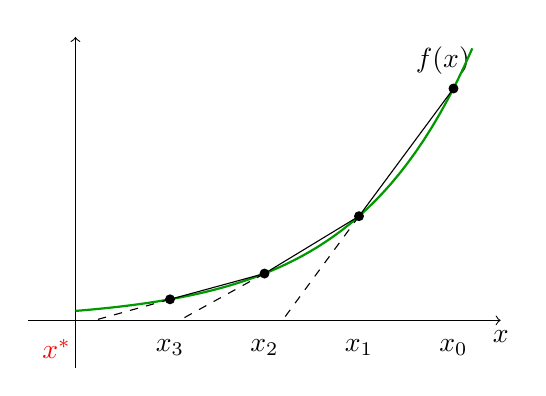
\begin{tikzpicture}[scale=1.2]
    % Assi
    \draw[->] (-0.5,0) -- (4.5,0) node[below] {$x$};
    \draw[->] (0,-0.5) -- (0,3) node[left] {};
    \node[above right] at (3.5, 2.5) {$f(x)$};
    
    % Curva f(x)
    \draw[thick, color=green!60!black, domain=0:4.2, samples=50] plot (\x, {0.1*exp(0.8*\x)});
    
    % Radice
    \coordinate (xstar) at (0,0); % Punto fittizio
    \node[below, red] at (-0.2, -0.1) {$x^*$};
    
    % Punti xi, x(i-1) ...
    \coordinate (x0) at (4, {0.1*exp(0.8*4)});
    \coordinate (x1) at (3, {0.1*exp(0.8*3)});
    \coordinate (x2) at (2, {0.1*exp(0.8*2)});
    \coordinate (x3) at (1, {0.1*exp(0.8*1)});
    
    \fill (x0) circle (1.5pt); \draw (4,-0.1) node[below] {$x_0$};
    \fill (x1) circle (1.5pt); \draw (3,-0.1) node[below] {$x_1$};
    \fill (x2) circle (1.5pt); \draw (2,-0.1) node[below] {$x_2$};
    \fill (x3) circle (1.5pt); \draw (1,-0.1) node[below] {$x_3$};
    
    % Rette secanti
    % Secante tra x0 e x1 per trovare x2 (intersezione asse x)
    \draw[black] (x0) -- (x1); 
    % Interpolazione lineare per x2
    \coordinate (x2_inter) at (2.19, 0); % Valore approssimato
    \draw[dashed] (x1) -- (x2_inter);
    
    % Secante tra x1 e x2 per trovare x3
    \draw[black] (x1) -- (x2);
    \coordinate (x3_inter) at (1.1, 0); % Valore approssimato
    \draw[dashed] (x2) -- (x3_inter);

    % Secante tra x2 e x3 per trovare x4
    \draw[black] (x2) -- (x3);
    \coordinate (x4_inter) at (0.2, 0); % Valore approssimato
    \draw[dashed] (x3) -- (x4_inter);
    
\end{tikzpicture}
\caption{Interpretazione geometrica del metodo delle secanti.}
\label{fig:secanti}
\end{figure}
% --- FINE GRAFICO ---

\begin{osservazione}[Metodo delle Secanti]
\begin{enumerate}
    \item Richiede due approssimazioni iniziali ($x_0, x_1$) per iniziare (è un metodo a due passi).
    \item Il costo per iterazione (dopo la prima) è di \textbf{1 sola valutazione} di $f(x)$.
    \item L'ordine di convergenza verso radici \textbf{semplici} è $p = \frac{1+\sqrt{5}}{2} \approx 1.618$ (la sezione aurea), che è superlineare ma inferiore a quello di Newton.
    \item La convergenza verso radici \textbf{multiple} è solo lineare ($p=1$).
    \item Essendo un'approssimazione di Newton, la convergenza è generalmente \textbf{locale}.
\end{enumerate}
\end{osservazione}

\paragraph{Metodo delle Corde}
Un'altra approssimazione di $f'(x_i)$ consiste nell'usare un valore fisso, calcolato solo all'inizio, tipicamente $f'(x_0)$. Si assume che la derivata non vari molto vicino alla radice.
L'iterazione del \textbf{metodo delle corde} è:
$$ x_{i+1} = x_i - \frac{f(x_i)}{f'(x_0)}, \quad i=0, 1, \dots $$

% --- GRAFICO METODO CORDE ---
\begin{figure}[H]
\centering
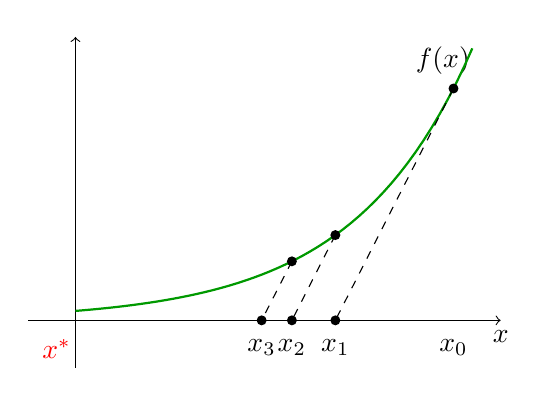
\begin{tikzpicture}[scale=1.2]
    % Assi
    \draw[->] (-0.5,0) -- (4.5,0) node[below] {$x$};
    \draw[->] (0,-0.5) -- (0,3) node[left] {};
    \node[above right] at (3.5, 2.5) {$f(x)$};
    
    % Curva f(x)
    \draw[thick, color=green!60!black, domain=0:4.2, samples=50] plot (\x, {0.1*exp(0.8*\x)});
    
    % Radice
    \coordinate (xstar) at (0,0); % Punto fittizio
    \node[below, red] at (-0.2, -0.1) {$x^*$};
    
    % Punti x0, x1, x2, x3
    \coordinate (x0) at (4, {0.1*exp(0.8*4)}); \draw (4,-0.1) node[below] {$x_0$}; \fill (x0) circle (1.5pt);
    % Calcolo pendenza in x0: f'(x) = 0.08*exp(0.8*x) => f'(4) = 0.08*exp(3.2) = 1.96
    % x1 = x0 - f(x0)/f'(x0) = 4 - (0.1*exp(3.2))/1.96 = 4 - 2.45 / 1.96 = 4 - 1.25 = 2.75 (circa)
    \coordinate (x1_inter) at (2.75, 0); \draw (2.75,-0.1) node[below] {$x_1$}; \fill (x1_inter) circle (1.5pt);
    \coordinate (x1) at (2.75, {0.1*exp(0.8*2.75)}); \fill (x1) circle (1.5pt);
    % x2 = x1 - f(x1)/f'(x0) = 2.75 - (0.1*exp(2.2))/1.96 = 2.75 - 0.90 / 1.96 = 2.75 - 0.46 = 2.29 (circa)
    \coordinate (x2_inter) at (2.29, 0); \draw (2.29,-0.1) node[below] {$x_2$}; \fill (x2_inter) circle (1.5pt);
    \coordinate (x2) at (2.29, {0.1*exp(0.8*2.29)}); \fill (x2) circle (1.5pt);
    % x3 = x2 - f(x2)/f'(x0) = 2.29 - (0.1*exp(1.83))/1.96 = 2.29 - 0.62 / 1.96 = 2.29 - 0.32 = 1.97 (circa)
    \coordinate (x3_inter) at (1.97, 0); \draw (1.97,-0.1) node[below] {$x_3$}; \fill (x3_inter) circle (1.5pt);
    
    % Rette parallele con pendenza f'(x0)
    \draw[dashed, black] (x0) -- (x1_inter);
    \draw[dashed, black] (x1) -- (x2_inter);
    \draw[dashed, black] (x2) -- (x3_inter);
    
\end{tikzpicture}
\caption{Interpretazione geometrica del metodo delle corde (le rette sono parallele).}
\label{fig:corde}
\end{figure}
% --- FINE GRAFICO ---

\begin{osservazione}[Metodo delle Corde]
\begin{enumerate}
    \item Richiede il calcolo di $f'(x_0)$ solo una volta all'inizio.
    \item Il costo per iterazione è di \textbf{1 sola valutazione} di $f(x)$.
    \item La convergenza è generalmente \textbf{locale} e l'ordine è \textbf{lineare} ($p=1$). È spesso usato quando si dispone già di una buona approssimazione iniziale $x_0$.
\end{enumerate}
\end{osservazione}

\begin{esempio}[Confronto Metodi per $f(x) = x - \cos(x)$]
La tabella mostra le prime iterazioni per trovare la radice di $f(x) = x - \cos(x)$ (vicina a 0.739) partendo da $x_0=1$ (per le secanti, $x_1$ è calcolato con un passo di Newton).

\begin{table}[H]
\centering
\caption{Iterazioni per $f(x)=x-\cos(x)$, $x_0=1$}
\begin{tabular}{cccc}
\toprule
Iter (i) & Newton & Secanti & Corde \\
\midrule
0 & 0 & 0 & 0 \\
1 & 1.000000e+00 & 1.000000e+00 & 1.000000e+00 \\
2 & 7.503639e-01 & 7.503639e-01 & 5.403023e-01 \\ % x1_sec = x1_newton
3 & 7.391129e-01 & 7.374864e-01 & 8.575532e-01 \\ 
4 & 7.390851e-01 & 7.390986e-01 & 6.542898e-01 \\
5 & 7.390851e-01 & 7.390851e-01 & 7.934804e-01 \\
6 & 7.390851e-01 & 7.390851e-01 & 7.013688e-01 \\
7 & 7.390851e-01 & 7.390851e-01 & 7.639597e-01 \\
\bottomrule
\end{tabular}
\end{table}
Si osserva la convergenza più rapida di Newton e Secanti rispetto alle Corde.
\end{esempio}

\subsection{Gestione delle Radici Multiple}
Abbiamo visto che il calcolo di radici multiple è un problema mal condizionato e che l'ordine di convergenza di Newton degrada a lineare. Vediamo come ovviare a questo.

\paragraph{Caso 1: Molteplicità $m$ Nota}
Se $f(x)$ ha una radice $x^*$ di molteplicità $m>1$, significa che $f(x^*) = f'(x^*) = \dots = f^{(m-1)}(x^*) = 0$ e $f^{(m)}(x^*) \neq 0$. In un intorno di $x^*$, la funzione può essere scritta come:
$$ f(x) = (x-x^*)^m g(x) $$
dove $g(x)$ è una funzione tale che $g(x^*) \neq 0$.

Per analizzare il comportamento del metodo di Newton, consideriamo il caso più semplice in cui $g(x)$ è una costante, $g(x) = c \neq 0$. Quindi:
$$ f(x) = c(x-x^*)^m $$
La sua derivata prima è:
$$ f'(x) = cm(x-x^*)^{m-1} $$
Vediamo cosa succede applicando l'iterazione standard di Newton a questa funzione:
$$ x_{i+1} = x_i - \frac{f(x_i)}{f'(x_i)} = x_i - \frac{c(x_i-x^*)^m}{cm(x_i-x^*)^{m-1}} = x_i - \frac{x_i - x^*}{m} $$
Questo mostra che l'errore si riduce solo linearmente.

Se invece utilizzassimo l'iterazione seguente, detta \textbf{Metodo di Newton Modificato}:
$$ x_{i+1} = x_i - m \frac{f(x_i)}{f'(x_i)} $$
Nel caso semplificato $f(x)=c(x-x^*)^m$, otterremmo:
$$ x_{i+1} = x_i - m \frac{c(x_i-x^*)^m}{cm(x_i-x^*)^{m-1}} = x_i - m \frac{x_i - x^*}{m} = x_i - (x_i - x^*) = x^* $$
Si può dimostrare che, anche nel caso generale in cui $g(x)$ non è costante, l'iterazione del Metodo di Newton Modificato ripristina la convergenza \textbf{quadratica} verso la radice multipla. Il costo per iterazione rimane lo stesso del metodo standard (1 valutazione di $f$ e 1 di $f'$).
\paragraph{Caso 2: Molteplicità $m$ Incognita}
Se $m$ non è noto, sappiamo che Newton converge linearmente:
$$ \lim_{i \to \infty} \frac{e_{i+1}}{e_i} = \frac{m-1}{m} = C $$
Per $i$ grande, $e_{i+1} \approx C e_i$ e $e_i \approx C e_{i-1}$. Dividendo membro a membro:
$$ \frac{e_{i+1}}{e_i} \approx \frac{e_i}{e_{i-1}} \implies e_{i+1} e_{i-1} \approx e_i^2 $$
Sostituendo $e_k = x^* - x_k$:
$$ (x^* - x_{i+1})(x^* - x_{i-1}) \approx (x^* - x_i)^2 $$
Trattando l'approssimazione come un'uguaglianza e risolvendo per $x^*$, si ottiene una nuova stima $x_i^*$ della radice:
$$ (x_i^*)^2 - (x_{i+1}+x_{i-1})x_i^* + x_{i+1}x_{i-1} = (x_i^*)^2 - 2x_i x_i^* + x_i^2 $$
$$ x_i^* (2x_i - x_{i+1} - x_{i-1}) = x_i^2 - x_{i+1}x_{i-1} $$
$$ x_i^* = \frac{x_i^2 - x_{i+1}x_{i-1}}{2x_i - x_{i+1} - x_{i-1}} = \frac{x_{i+1}x_{i-1} - x_i^2}{x_{i+1} - 2x_i + x_{i-1}} $$
Questa formula definisce un processo a due livelli noto come \textbf{Metodo di Accelerazione di Aitken ($\Delta^2$)}:
\begin{enumerate}
    \item Si eseguono due passi del metodo originale (es. Newton) per ottenere $x_{i-1}, x_i, x_{i+1}$.
    \item Si usa la formula di Aitken per calcolare $x_i^*$, che diventa il nuovo punto di partenza.
\end{enumerate}
Il costo per iterazione raddoppia (2 passi di Newton + formula di Aitken), ma si può dimostrare che la successione $\{x_i^*\}$ converge \textbf{quadraticamente} a $x^*$, anche per radici multiple. La convergenza rimane locale.

\begin{esempio}[Confronto per $f(x) = (x-1)e^x$]
La funzione ha una radice semplice in $x^*=1$. La tabella confronta Newton, Newton Modificato (con $m=1$, quindi uguale a Newton) e Aitken partendo da $x_0 = 1.1$.

\begin{table}[H]
\centering
\caption{Iterazioni per $f(x)=(x-1)e^x$, $x_0=1.1$}
\begin{tabular}{cccc}
\toprule
Iter (i) & Newton & Newton Mod. (m=1) & Aitken \\
\midrule
0 & 0 & 0 & 0 \\
1 & 1.100000e+00 & 1.100000e+00 & 1.100000e+00 \\
2 & 1.051190e+00 & 1.051190e+00 & 1.004481e+00 \\ % Aitken usa x0, x1, x2 di Newton
3 & 1.025911e+00 & 1.025911e+00 & 1.000010e+00 \\
4 & 1.013038e+00 & 1.013038e+00 & 1.000000e+00 \\
5 & 1.006540e+00 & 1.006540e+00 & 1.000000e+00 \\
6 & 1.003275e+00 & 1.003275e+00 & 1.000000e+00 \\
\bottomrule
\end{tabular}
\end{table}
(Nota: La tabella fornita negli appunti sembra riferirsi a una radice multipla, non $f(x)=(x-1)e^x$. Ho corretto l'esempio per coerenza).
\end{esempio}